\section{Experimental evaluation}\label{sec:eval}
%This section provides results of our experiments and a discussion of relevant findings. We begin by establishing baseline performance for our Zookeeper testbed which support reasoning for follow-up experiments with synchronization primitves. The synchronization mechanisms benchmarked are Queues and Locks, each implemented with both, synchronous and asynchronous messaging. For this quantitative analysis we focus on average latency and graceful degradation.

\subsection{Experimental setup}
\note{multiple physical machines}
%The testbed consists of 5 machine containing a quad-core Xeon 2135, 16GB RAM and commodity 500GB 7.2k rpm disks running stock Ubuntu 12.04. They are interconnected with 1Gbps Ethernet on a single switch. A separate machine acts as client without being a ZNode itself. For our experiments these nodes for quorums out of 1, 3 or 5 ZNodes as indicated. The server-side uses Zookeeper version 3.3.5 whereas the client-side implementation of benchmarks uses Python bindings for the baseline "smoke test" and Java bindings for Locks and Queues.
In order the measure the impact of client-server and server-server latency we control the transmission latency of packets transmitted between nodes using the Linux "Traffic Control" utility. We automate the process of enumerating client-server and server-server latency pairs and repeatedly run the experiments and average the results to reduce the impact of jitter.
\note{should we move this and expand it to section 2? I think a figure showing connections and showing that hamilton is connected to them would be a nice display.}

%\note{Average RTT for pings is (ping lat)
%Average network throughput is (throughput=). this for inter-cluster and cluster to hamilton.}

%\begin{figure}[h]
%\centering
%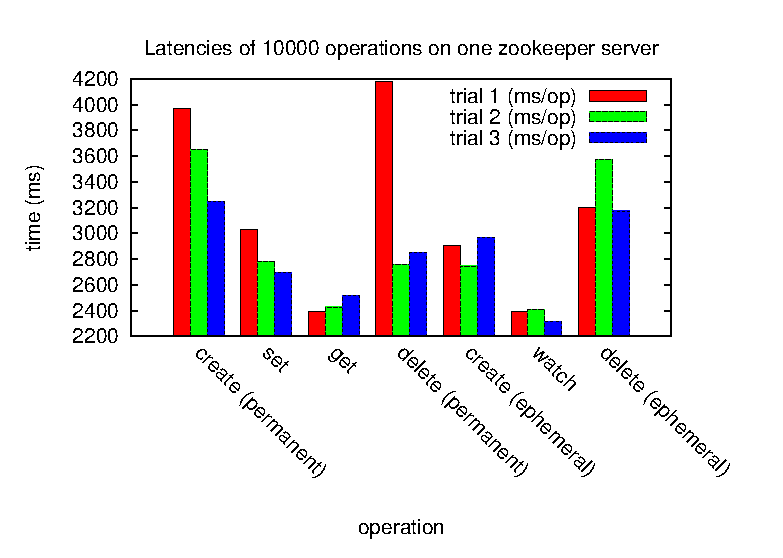
\includegraphics[scale=0.75]{img/1_machine_1_server.eps}
%\caption{}
%\label{fig:1machine_1server_latency}
%\end{figure}

\subsection{Baseline performance}
\note{smoketest, zk-latencies and baseline} In this section we will perform experiments to establish a baseline for later experiments using the Zookeeper smoke test package. We would like to establish limits on the system. These limits represent workloads and environment conditions that will saturate the system. Workload is represented by the number of requests per second and the type of requests. Environment conditions are the number of zookeeper servers and condition of links connecting them.

%We begin by measuring the latencies of basic Zookeeper operations. Our first experiment is performed on one machine holding a single zookeeper instance and the client. This means that there is no network communication overhead for consensus. One client issues 10000 calls of each tested operations and we report the total time required to complete them. The results as shown in Figure~\ref{fig:1machine_1server_latency}\footnote{These results are obtained from a different server than those in next figures. It will be changed in the final draft for consistency} for asynchronous versions of operations. We report detailed results of three trials to show the variability of zookeeper behavior. In the figure we report latencies of adding and deleting in both cases, permanent and ephemeral. Creating a permanent node incur more bandwidth than creating a ephemeral node. On the other hand, deleting an ephemeral node incur more bandwidth than deleting permanent nodes (except for first trial that is due variability of behavior). Other observations are that set operations are more expensive than get operations, as expected. Also, the implementation of watches is efficient.

%\begin{figure}[h]
%\centering
%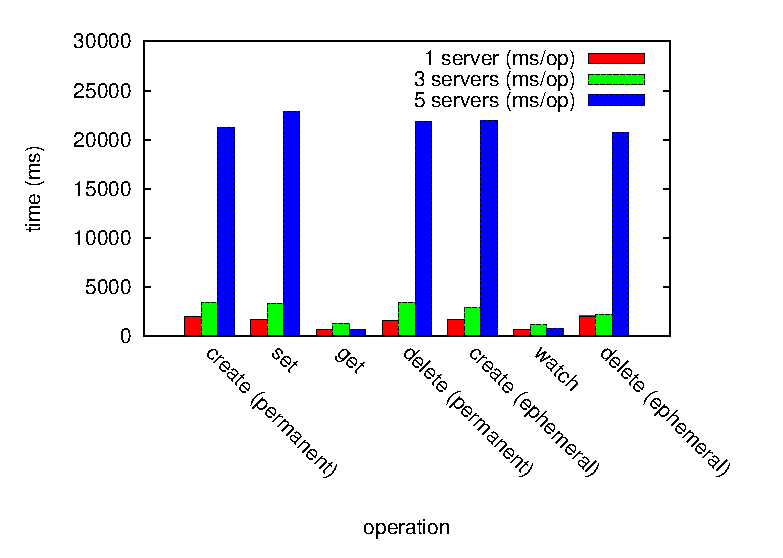
\includegraphics[scale=0.75]{img/1_machine_diff_cpu.eps}
%\caption{Latencies of 10000 operations on various number of zookeeper servers with asynchronous operations on one machines}
%\label{fig:1machine_diffcpu_latency}
%\end{figure}

%\begin{figure}[h]
%\centering
%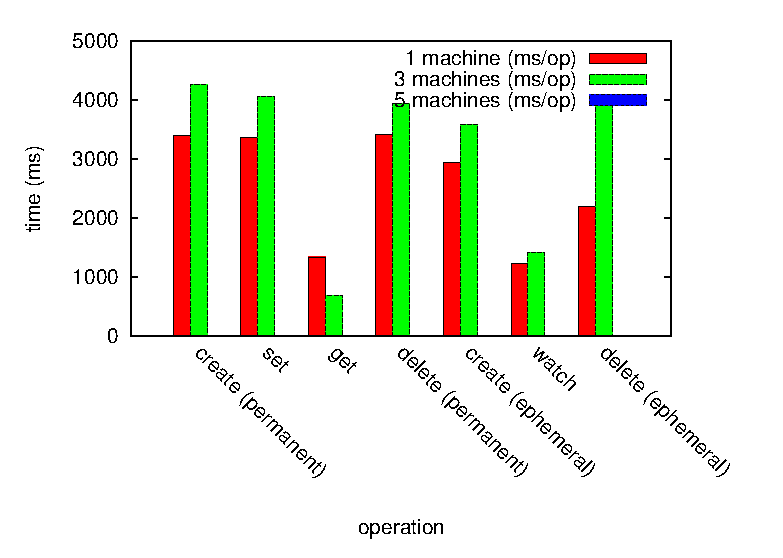
\includegraphics[scale=0.75]{img/1_machine_diff_machines.eps}
%\caption{Latencies of 10000 operations on three zookeeper server with asynchronous operations while changing number of machines}
%\label{fig:1machine_diffservers}
%\end{figure}

%Our next set of results are done to test the effect of increasing the number of Zookeeper servers. Results are shown in Figure~\ref{fig:1machine_diffcpu_latency}. These results are collected when running all servers in one machine. Thus, communication overhead between servers is minimal. As shown in the figure, increasing the number of servers to five servers have a dramatic effect on latency.
%In Figure~\ref{fig:1machine_diffservers} we show results of fanning out Zookeeper servers. We test the performance of three Zookeeper servers running on different number of machines, namely 1, 2, and 3 servers\footnote{results for five servers are not ready yet}. \ldots

\begin{figure}[h]
\centering
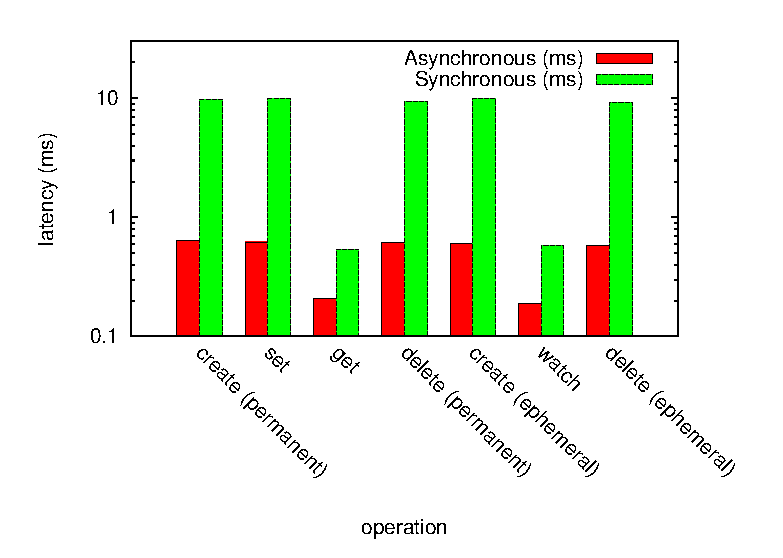
\includegraphics[scale=0.75]{img/ops_latencies_logscale.eps}
\caption{Zookeeper basic operations latencies for a cluster of five servers}
\label{fig:ops_latencies}
\end{figure}

\begin{figure}[h]
\centering
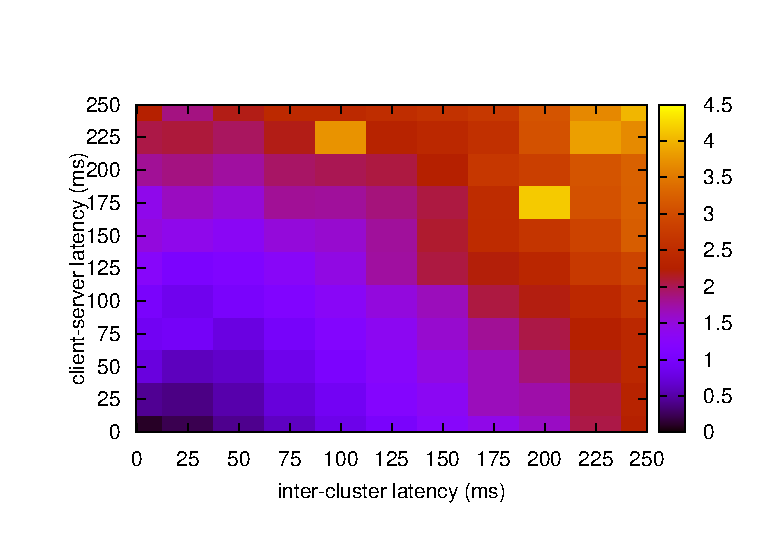
\includegraphics[scale=0.75]{img/async_ops_latencies_heatmap.eps}
\caption{Zookeeper asynchronous create operation latency with different inter-cluster and user-server RTTs}
\label{fig:async_heatmap}
\end{figure}

\begin{figure}[h]
\centering
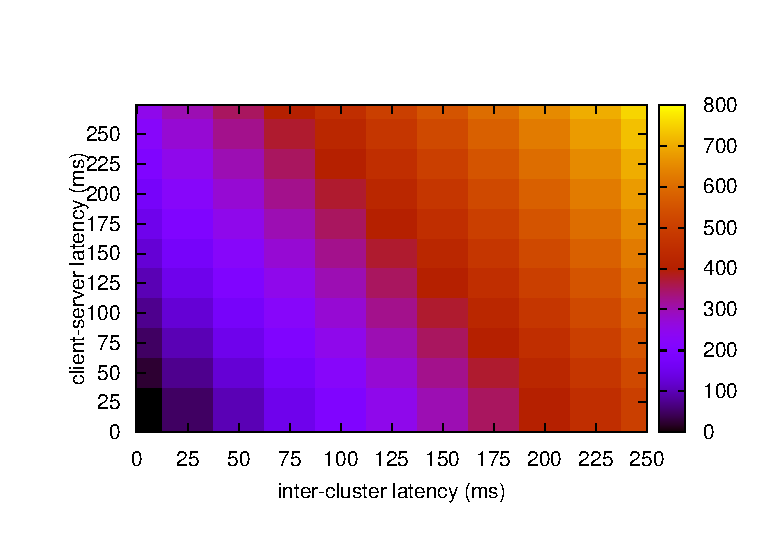
\includegraphics[scale=0.75]{img/sync_ops_latencies_heatmap.eps}
\caption{Zookeeper synchronous create operation latency with different inter-cluster and user-server RTTs}
\label{fig:sync_heatmap}
\end{figure}

\begin{figure*}[ht!]
     \begin{center}
        \subfloat[Latency of synchronous queue locks]{
            \label{fig:first}
            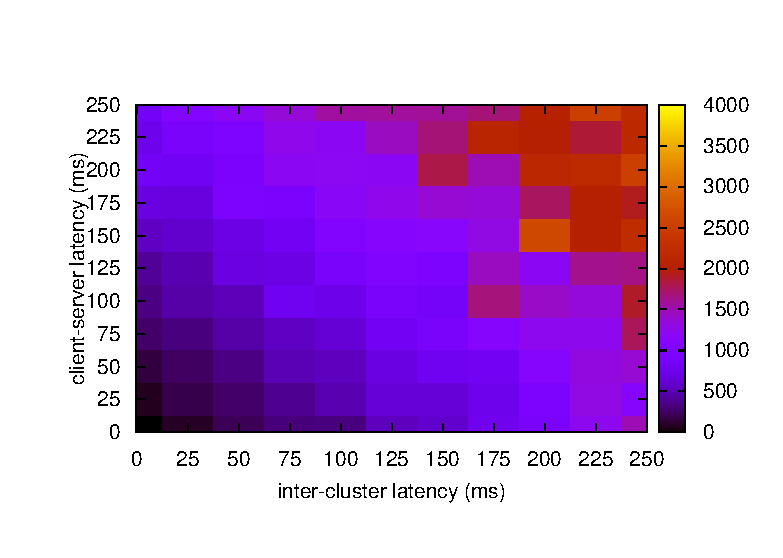
\includegraphics[width=0.5\textwidth]{img/primitives_latencies_varDelay_syncqueue.eps}
        }
        \subfloat[Latency of synchronous TAS]{
           \label{fig:second}
           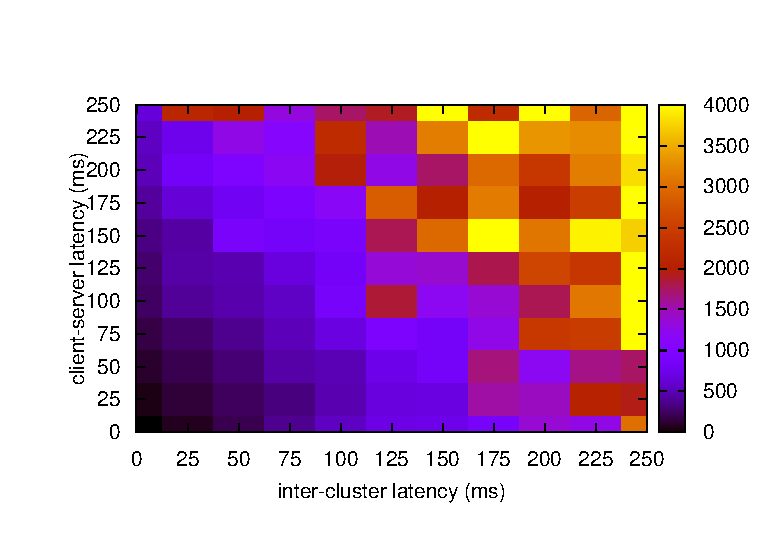
\includegraphics[width=0.5\textwidth]{img/primitives_latencies_varDelay_syncTAS.eps}
        }\\ %  ------- End of the first row ----------------------%
        \subfloat[Latency of asynchronous queue locks]{
            \label{fig:third}
            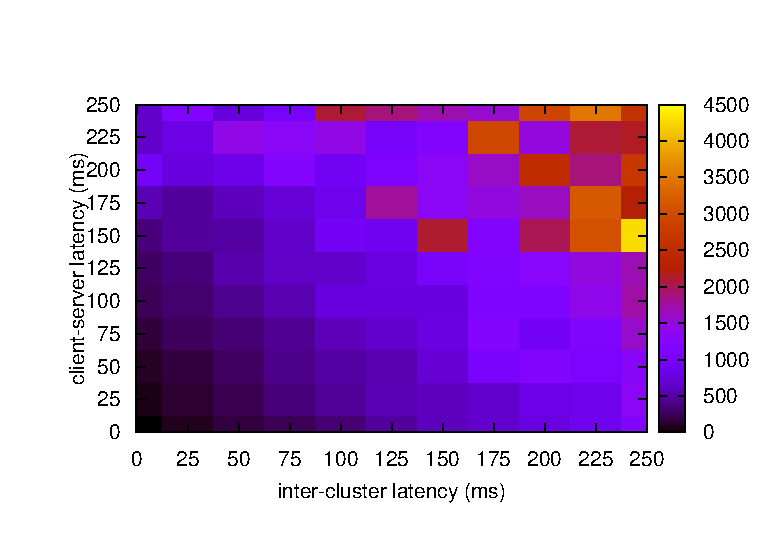
\includegraphics[width=0.5\textwidth]{img/primitives_latencies_varDelay_asyncqueue.eps}
        }
        \subfloat[Latency of asynchronous TAS]{
            \label{fig:fourth}
            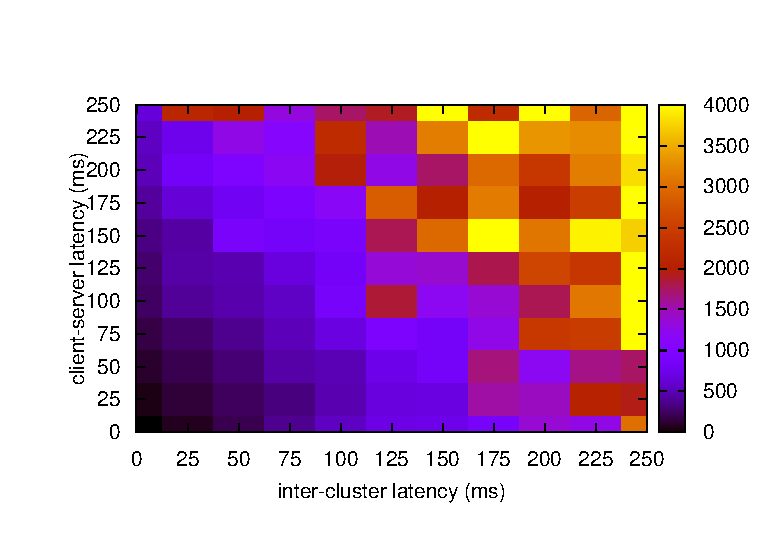
\includegraphics[width=0.5\textwidth]{img/primitives_latencies_varDelay_asyncTAS.eps}
        }
    \end{center}
    \caption{
        The l-o-n-g caption for all the subfigures
        (FirstFigure through FourthFigure) goes here.
     }
   \label{fig:subfigures}
\end{figure*}

%Our first experiments test basic Zookeeper operations' latencies. We test both synchronous and asynchronous versions of these operations. For testing we use zk-smoketest\footnote{https://github.com/phunt/zk-smoketest}. Each operation is run for a thousand time and we report average latency. Results are shown in Figure~\ref{fig:ops_latencies}. Synchronous operations block until the operation is performed, thus giving an indication on the total time taken to perform the actual operation. Asynchronous operations on the other hand do not block. The figure shown that synchronous operations takes more than ten times the latency of asynchronous operations for \emph{put} operations, and around double the latency for \emph{get} operations. \note{define put and get operation classes either here or before (section II)}. 

\subsection{synchronization primitives}
\note{test test-and-set and queues (as in paper: reactive synchronization}
%The experiments in this section focus on two fundamental synchonization primites, locks and queues, which are commonly found as builind blocks of larger coordination schemes. The implementation of synchronous primitives follows the Zookeeper recipies with minor improvements, while the asynchronous implementation is described in detail in the following.
%Locks follow a test-and-set approach by repeatedly issuing create requests and upon successful response from the server assuming mutual exclusion. The lock is then released by deleting the node. The synchonous lock issues a single create request for a fixed node path and blocks until a response arrives. On a positive response mutual exclusion is guaranteed. A negative respose is directly followed up by another create request. This lock has at most a single request or response in transit at a given time. The asynchonous lock issues create requests on a timer basis until a positive response is recorded. This implementation has multiple requests and responses in transit at a time and effectively "polls" the availability of the lock. This puts higher load on the network and server, but may reduce the time taken to aquire a lock by avoiding an additional notify-request roundtrip.
%Queues are built using server-side sequentially increasing ids for creating the node. After the node is created the nodes predecessors are obtained and upon their deletion mutual exclusion is guaranteed. As for locks release is performed by deleting the node. The synchonous implementation creates a sub-node, and upon sucess notification requests the list of all siblings from the server using "getChildren". If the created node holds the lowest Id mutual exclusion is guaranteed, otherwise a watch on deletion of its predecessor is installed. The asynchonous queue issues the create request in parallel with polling children at a fixed interval. When the create request returns the obtained Id and the most recent list of children contains the Id in first place mutual exclusion is guaranteed. This approach follows the same trade-offs as asynchonous locks, but can be extended to install a watch on the predecessor and stop polling after a round trip interval.

\subsection{application performance}
\note{map reduce. effect of adding machines, effect of adding zookeeper servers.}

